\chapter{Scheduling delle attività}
\section{Tabella di scheduling}
%
%	tabella di scheduling
%
\clearpage
\section{Work Breakdown Structure (WBS)}
In questa sezione è presentata la WBS del progetto e le WBS dettagliate per RAD, ODD e documentazione di testing; in particolare, per le WBS della documentazione vengono presentati due formati: l'org-chart format e l'outline format.

Nell'org-chart format vengono rappresentate le componenti principali che sono dettagliate nell'outline format per questione di spazio.
\subsection{WBS progetto}
\begin{figure}[ht]
\centering
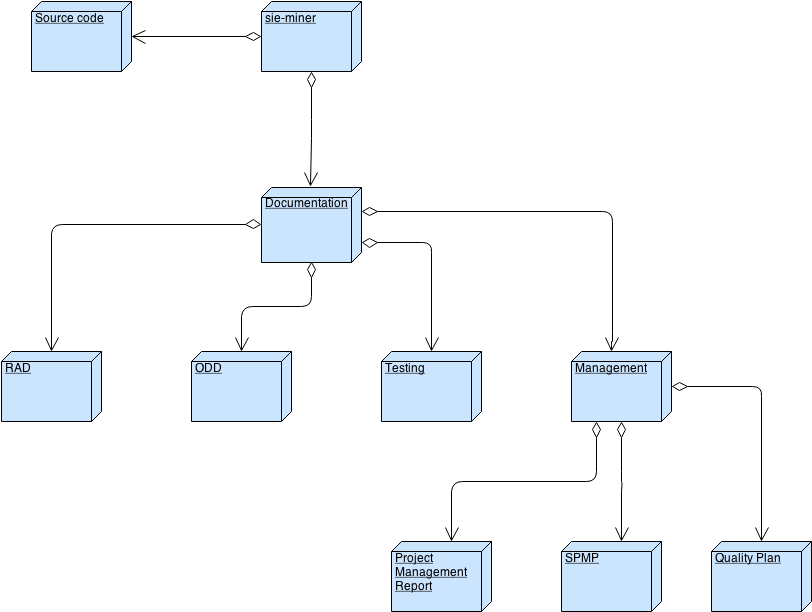
\includegraphics[width=\textwidth]{img/WBS_master.png}
\caption{WBS sie-miner} 
\end{figure}
\clearpage

% WBS RAD ---------------------

\subsection{WBS RAD}
\begin{figure}[ht]
\centering
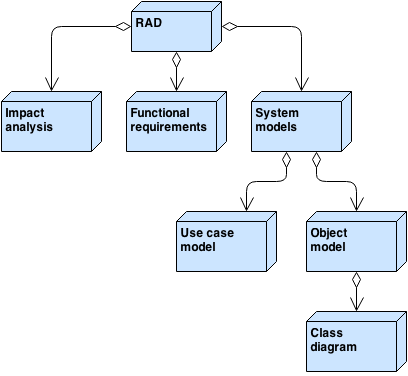
\includegraphics[width=.5\textwidth]{img/wbs_rad.png}
\caption{WBS RAD} 
\end{figure}
\textbf{WBS RAD - Outline format:}
\begin{enumerate}
\item Introduzione
\begin{enumerate}[label*=\arabic*.]
\item Scopo del sistema
\item Definizioni, acronimi, abbreviazioni
\item Panoramica
\item Sistema corrente
\end{enumerate}
\item Sistema proposto
\begin{enumerate}[label*=\arabic*.]
\item Requisiti funzionali
\end{enumerate}
\item System Model
\begin{enumerate}[label*=\arabic*.]
\item Use case models
\item Object models
\end{enumerate}
\item Glossario
\end{enumerate}
\clearpage

% WBS ODD ---------------------
\subsection{WBS ODD}
\begin{figure}[ht]
\centering
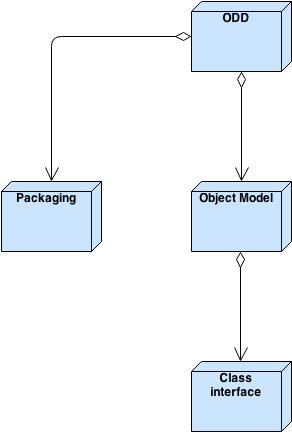
\includegraphics[width=.5\textwidth]{img/ODD.png}
\caption{WBS ODD} 
\end{figure}
\textbf{WBS ODD - Outline format:}
\begin{enumerate}
\item Introduzione
\begin{enumerate}[label*=\arabic*.]
\item Trade off dell'object design
\item Linee guida per la documentazione delle interfacce
\item Definizioni, acronimi e abbreviazioni
\item References
\end{enumerate}
\item Package
\begin{enumerate}[label*=\arabic*.]
\item Package
\item Comunicazione tra i package
\item Classi e interfacce nei package
\end{enumerate}
\item Object Model
\begin{enumerate}[label*=\arabic*.]
\item Interfaccia delle classi
\end{enumerate}
\item Glossario
\end{enumerate}
\clearpage

% WBS testing ---------------------
\subsection{WBS testing}
\begin{figure}[ht]
\centering
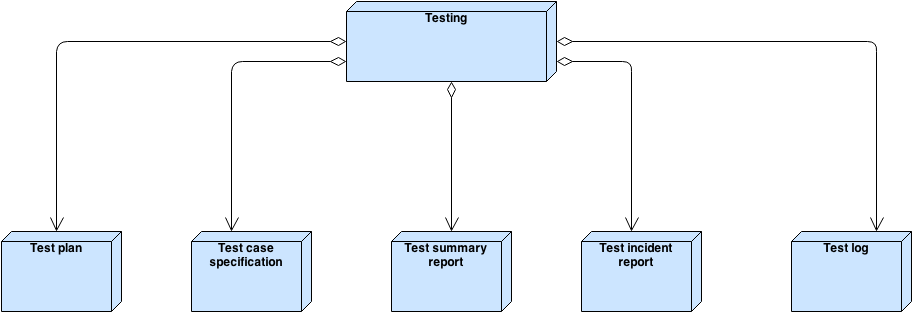
\includegraphics[width=\textwidth]{img/WBS_testing.png}
\caption{WBS Testing} 
\end{figure}
\textbf{WBS ODD - Outline format:}\\ \\
\textbf{Test Plan}:
\begin{enumerate}
\item Introduzione
\item Relazioni con altri documenti
\item Panoramica del sistema
\item Funzionalità da testare/non testare
\item Pass/Fail criteria
\item Approccio
\item Sospensione e ripristino
\item Strumenti per il testing (Hardware e software)
\item Test case
\item Pianificazione del test
\end{enumerate}
\clearpage

\section{Diagramma di Gantt}